%-------------------------------------------------------------------------------
%	NAME:	report.tex
%	AUTHOR: Connor Beardsmore - 15504319
%	LAST MOD:	18/09/16
%	PURPOSE:	CG Assignment 2 Report
%	REQUIRES:	NONE
%-------------------------------------------------------------------------------

\documentclass[]{article}
\usepackage[ margin=3cm ]{geometry}
\usepackage{graphicx}
\usepackage{fancyhdr}
\usepackage{float}
\usepackage{hyperref}
\usepackage{transparent}
\usepackage[style=chicago-authordate,backend=biber]{biblatex}


\pagestyle{fancy}
\fancyhf{}
\lhead{Connor Beardsmore - 15504319}
\rhead{CG200}
\lfoot{October 2016}
\rfoot{\thepage}

\pagenumbering{arabic}
\graphicspath{{./images/}}

\addbibresource{./references.bib}
\nocite{*}



%-------------------------------------------------------------------------------
\begin{document}
%-------------------------------------------------------------------------------

\begin{titlepage}
	\begin{center}
		\vspace*{1cm}
		\LARGE\textbf{CG200 Report}
		\break
		OpenGL Assignment
		\vspace{1cm}
		\break
		\Large\textbf{Connor Beardsmore - 15504319} 

		\vspace{1cm}
		\begin{figure}[H]
			\begin{center}
				{\transparent{0.2} 
					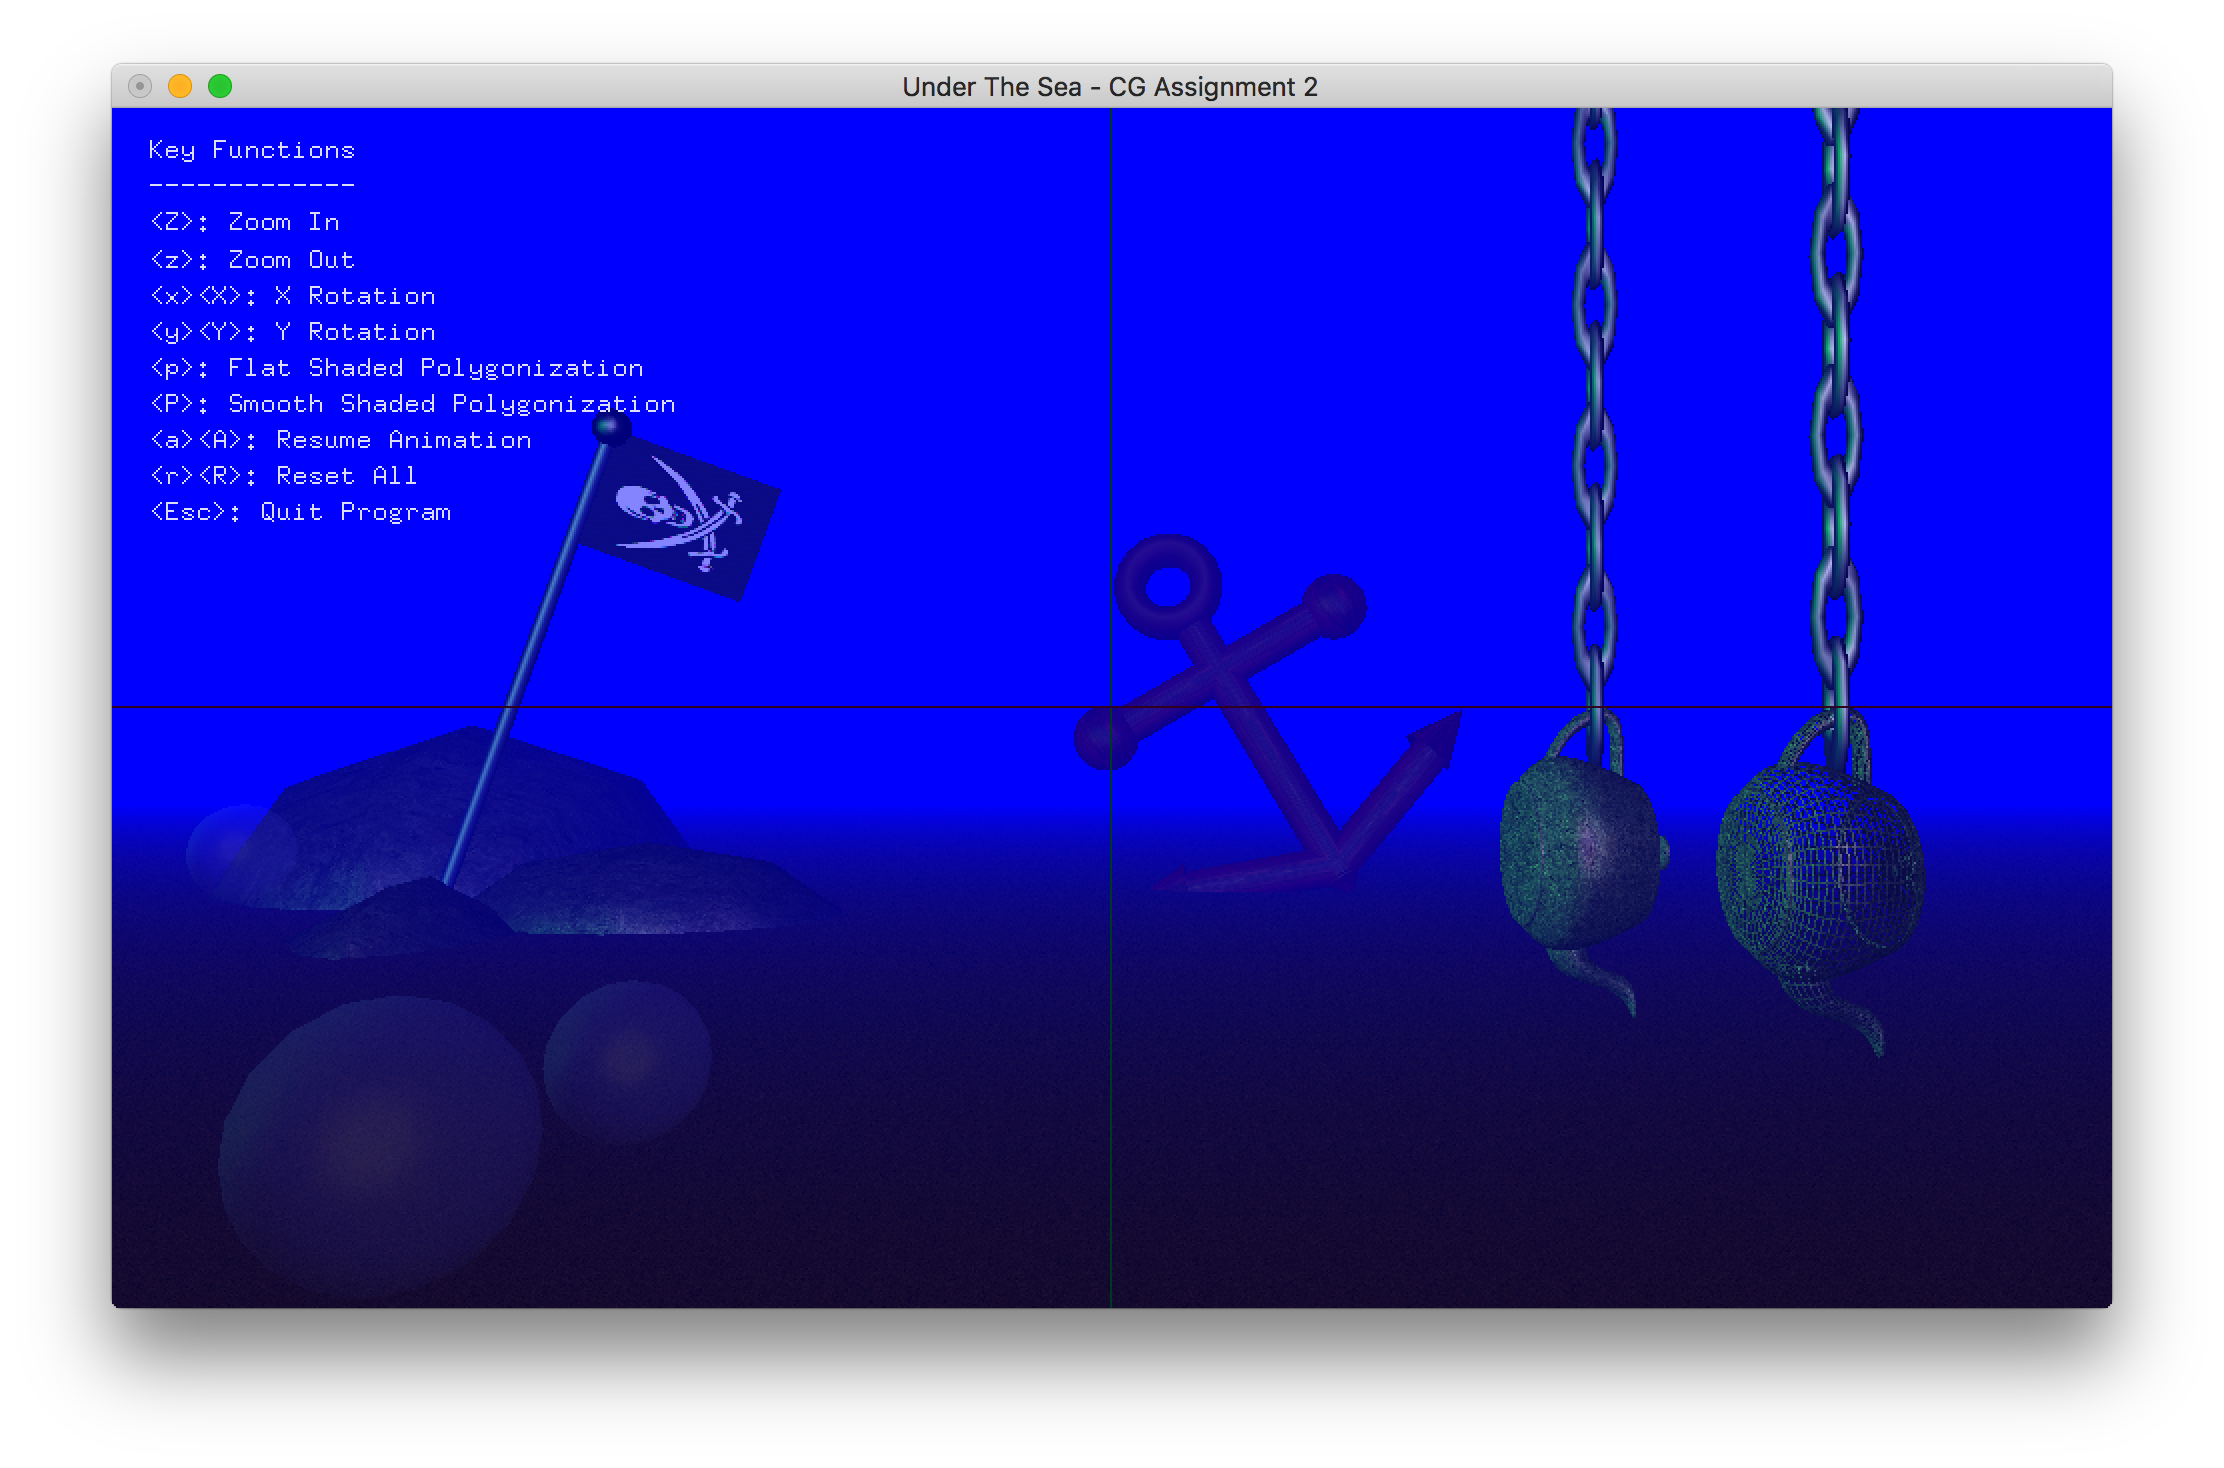
\includegraphics[height=0.5\textheight,width=\textwidth]{scene.png}}
			\end{center}
		\end{figure}

		\vspace{2cm}
		\normalsize
		Curtin University \\
		Science and Engineering \\
		Perth, Australia \\
	    October 2016
	    
	\end{center}
\end{titlepage}

%-------------------------------------------------------------------------------

\vspace*{-0.8cm}
\begin{center}
	\section*{OpenGL \textquotedblleft Under The Sea\textquotedblright Assignment}
\end{center}

%-------------------------------------------------------------------------------

\vspace*{0.8cm}
\section*{Features Implemented}

All features specified by the marking guide have been implemented and the scene consists of the following features. Key press functions have been utilized to allow the user to control the scene with the keyboard. The keys and instructions to run are clearly illustrated in the scene. A basic animation has been developed, with full details of this described later in the report. Each shape becomes clearly the closer you zoom, with level-of-details clarity performed. To increase realism, several objects have a combination of both texture maps and surface finishes. Two coloured light sources are located in the front and rear of the scene, with the specular surface finishes showing realistic highlights on the object surfaces. The use of additional effects has also been applied, with the bubbles illustrating transparency and the entire scene being enveloped in light blue fog.

%-------------------------------------------------------------------------------

\section*{Main Algorithms}

\begin{itemize}
	\item how was chain created
	\item how was anchor created
	\item how does fog work 
	\item level of details 
	\item all ojects take in x,y,z for easy movement
	\item push and pops
\end{itemize}

%-------------------------------------------------------------------------------

\section*{Objects Modelled and Surface Finishes}

The scene consists of multiple shapes, both simple and composite. The floor was modelled as a simple square plane, with a basic "dirt" bitmap for it's texture mapping. Three rock objects were created via calls to gluSphere(). These rocks also utilized a texture map to provide additional realism. Further spheres were employed for use in the three transparent bubbles on the left of the scene. These spheres vary in size with transparency to correlate with real bubbles. While appearing complex, the teapots are actually created through the GLUT library, with calls to glutSolidTeapot(). The teapot is the only object in the GLUT library that allows for texture mapping and thus, a "brass" texture map was applied to the teapots. The use of material surface finishes creates the appearance that the teapot is old, mouldy and rusted. \\

The composite objects are the teapot chain, the pirate flagpole and the wooden anchor. These three composite objects use combinations of various simple objects such as spheres, torus, cylinders and cones to a varying degree of complexity. The teapot chain is simply a torus, scale and stretched. The torus is repeatedly created in a for loop, with each alternative object being rotated at a 90 degree angle to the previous. The flagpole consists of a sphere top, cylinder pole and flat plane for the flag.

// TALK ABOUT ANCHOR HERE
%-------------------------------------------------------------------------------

\section*{External Tools}

No external tools were utilized for the scene. All composite objects were modelled within the code with no external assistance. More complex composite objects could have been converted from .obj files, but it was a stronger learning experience to create these objects myself through trial and error techniques.

%-------------------------------------------------------------------------------

\section*{Animation}

\begin{itemize}
	\item flag pole sinks into ground
	\item bubbles translate up,right and back into the distance
	\item teapot chain mvoes up and rotates 
	\item fog moves forwards/backwards over time
\end{itemize}

%-------------------------------------------------------------------------------

\break
\setlength\bibitemsep{4\itemsep}
\printbibliography

%-------------------------------------------------------------------------------
\end{document}   
%-------------------------------------------------------------------------------